\section{Tracking}

The drift chamber, with 112 layers of wires, provides high number of measurements which can be exploited for the track reconstruction.

One of the methods we are investigated is the Hough transform as described below.

\subsection{The Hough Transform}
Initially invented for bubble chamber photographs~\cite{HTWikipedia}, the Hough Transform is a feature extraction technique used in several fields such as image analysis, computer vision and digital image procession. It allows for the identification of lines as well as other shapes such as circles or ellipses.

\subsubsection{Principle}
The simplest case of Hough transform is detecting straight lines. In the parameter space, lines are represented as a point (b, m) with \cref{lineeq}.

\begin{equation}
	y = m \cdot x + b
	\label{lineeq}
\end{equation}

\begin{figure}[ht]
	\begin{tikzpicture}[scale=1.5]
    % Draw axes
    \draw [<->,thick] (0,2) node (yaxis) [above] {$y$}
        |- (3,0) node (xaxis) [right] {$x$};
    % Draw two intersecting lines
    \draw (0,0) coordinate (a_1) -- (2, 2) coordinate (a_2);
    \draw (0,1.5) coordinate (b_1) -- (1.8,0) coordinate (b_2);

    \coordinate (c) at (intersection of a_1--a_2 and b_1--b_2);
		% right angle
    \fill[red] (c) circle (2pt);

\end{tikzpicture}
\caption{TODO: A line is representate as a point (b, m) in the parameter space according to \cref{lineeq}.}
\label{fig_lineParamSpace}
\end{figure}

With the presentation (b, m) in the parameter space, vertical lines pose problems for the unbounded slope parameter \textit{m}. The Hesse normal form as described in \cref{line_hesse} can be used as a solution to get around vertical lines, where $r$ is the shortest distance from the origin to the line and $\theta$ is the angle between the $x$ axis and the line connecting the origin with the closest point as illustrated in \cref{fig_lineParamSpace}. The (r,~$\theta$) plane is referred to as the Hough Space.


\begin{equation}
	r = x \cdot \cos(\theta) + y \cdot \sin(\theta)
	\label{line_hesse}
\end{equation}

\cref{HTLine} shows the Hough transformation applied to every point on a line. In the Hough space, all the points on the line are represented by a local maximum since they all have the same (r,~$\theta$) value.
\begin{figure}[ht]
	\centering
	\begin{subfigure}[b]{0.45\textwidth}
        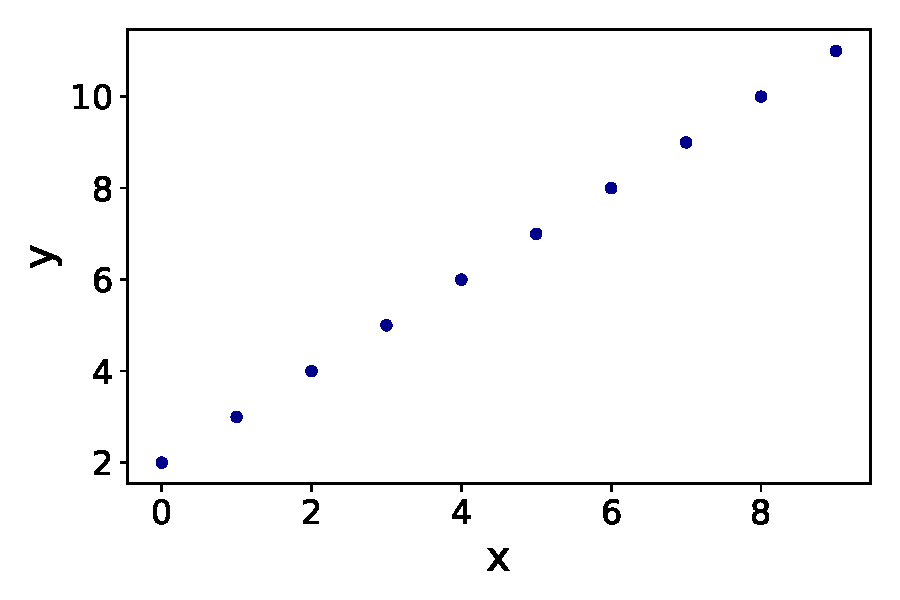
\includegraphics[width=\textwidth]{figures/line.pdf}
        \caption{Parameter space}
        % \label{pointsLine}
    \end{subfigure}
		~ %
		\begin{subfigure}[b]{0.45\textwidth}
					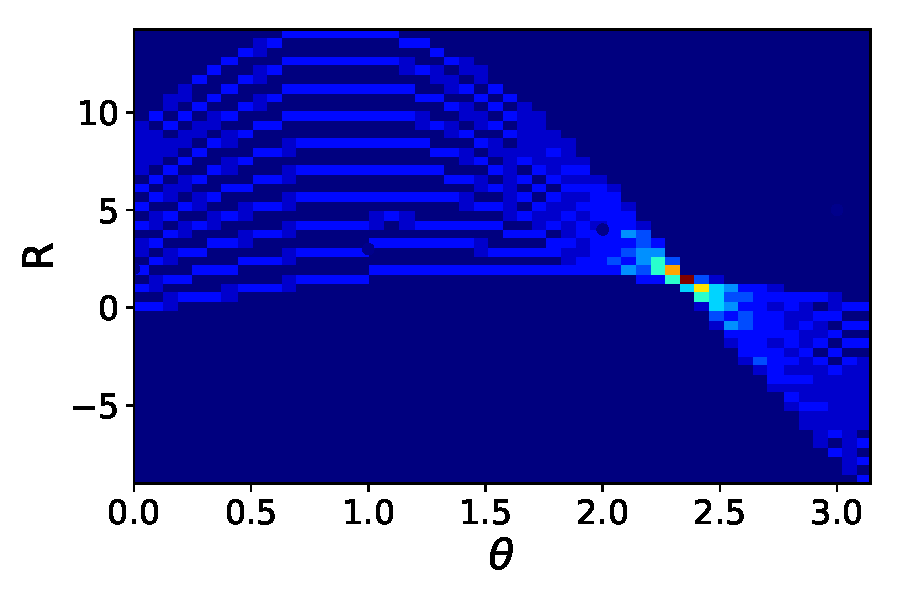
\includegraphics[width=\textwidth]{figures/line_hough.pdf}
					\caption{Hough space}
					% \label{pointsLine2}
			\end{subfigure}
	\label{HTLine}
	\caption{A line as represented in the parameter and the Hough space.}
\end{figure}

\subsubsection{Identification of circles}

The track of a charged particle in a magnetic field follows a helicoidal trajectory. In the xy-plane, the hits follow a circular trajectory as described with \cref{circleEq} where $(a, b)$ represent the center of the circle and $R$ the radius of the circle.

\begin{equation}
  {(x-a)}^2 + {(y-b)}^2 = R^2
	\label{circleEq}
\end{equation}

The Hough transformation gets better results when applied to lines. For this reason, first the conformal mapping~\cite{Hansroul:1988wa} is first applied to map circular hits into lines using \cref{conformalTrans}.

\begin{equation}
  u = {{x} \over {x^2+y^2}} , \,\,\,\, v = {{y} \over {x^2+y^2}}
	\label{conformalTrans}
\end{equation}

The conformal mapping maps a circle to a line if and only if the circle passes from the origin or following the condition as described in \cref{conformalTrans_condition} and the straight lines are described by \cref{equation_straightLine}.

\begin{equation}
  a^2 + b^2 = R^2
	\label{conformalTrans_condition}
\end{equation}

\begin{equation}
  v = {1 \over {2b}} - u {a \over b}
	\label{equation_straightLine}
\end{equation}

If the condition in \cref{conformalTrans_condition} is not satisfied, some correction terms are needed for the transformation in \cref{conformalTrans} to transform circles into lines.

The Hough transformation is then applied to the straight lines using \cref{Eq_HT_circle}.

\begin{equation}
	\rho = u \cdot cos(\phi) + v \cdot sin(\phi)
	\label{Eq_HT_circle}
\end{equation}

The radius of the circle $R$ is connected the $\rho$ parameter of the Hough transformation by \cref{Eq_R_rho}.

\begin{equation}
	R = {1 \over {2 \cdot \rho}}
	\label{Eq_R_rho}
\end{equation}

Finally, the center of the circle is extracted from the Hough transformation using \cref{Eq_HT_centers}.


\begin{equation}
	a = {cos(\phi) \over {2 \cdot \rho}},
\,\,\,\,
	b = {sin(\phi) \over {2 \cdot \rho}}
\label{Eq_HT_centers}
\end{equation}


\begin{figure}[ht]
	\centering
	\begin{subfigure}[b]{0.3\textwidth}
        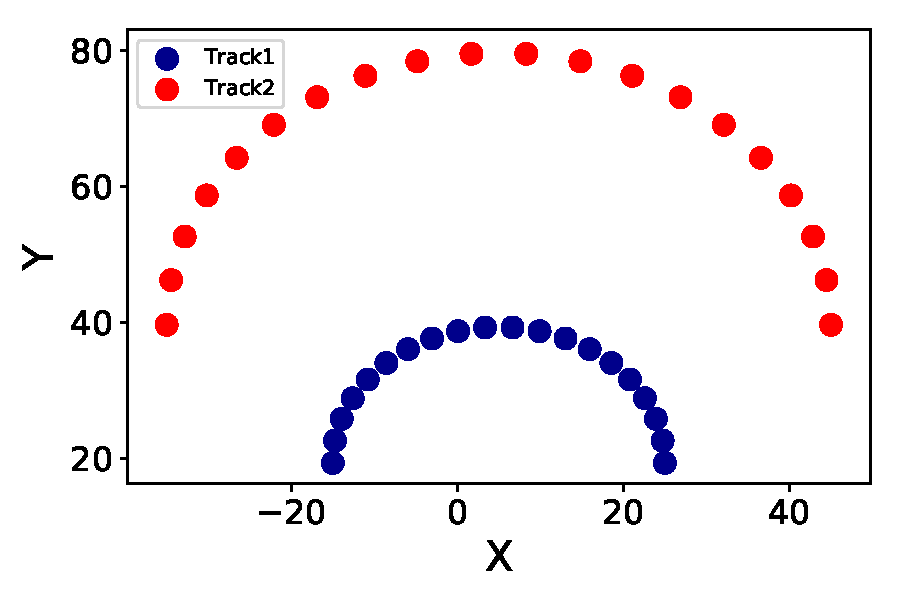
\includegraphics[width=\textwidth]{figures/circle.pdf}
        \caption{}

    \end{subfigure}
		~ %
		\begin{subfigure}[b]{0.3\textwidth}
					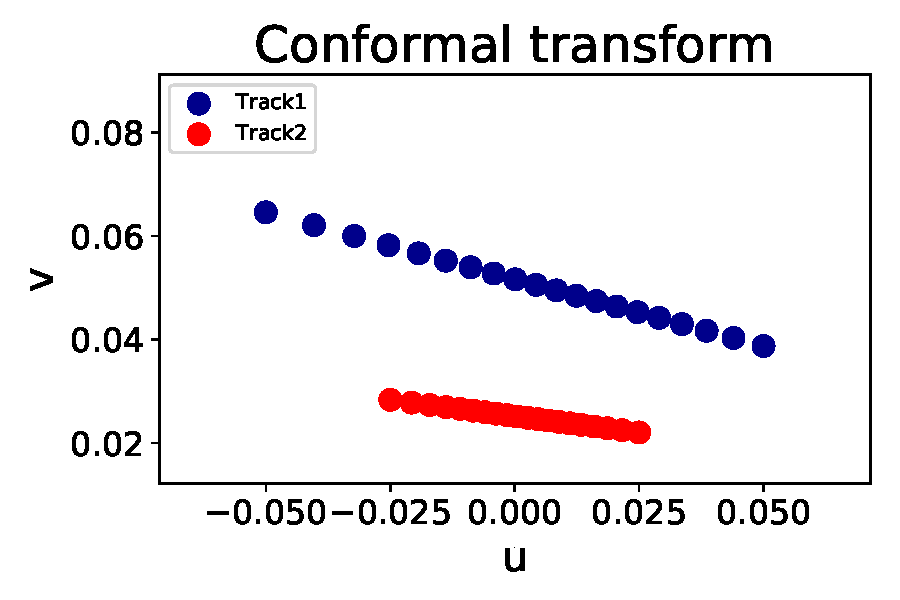
\includegraphics[width=\textwidth]{figures/circle_CT.pdf}
					\caption{}
			\end{subfigure}
			~ %
			\begin{subfigure}[b]{0.3\textwidth}
						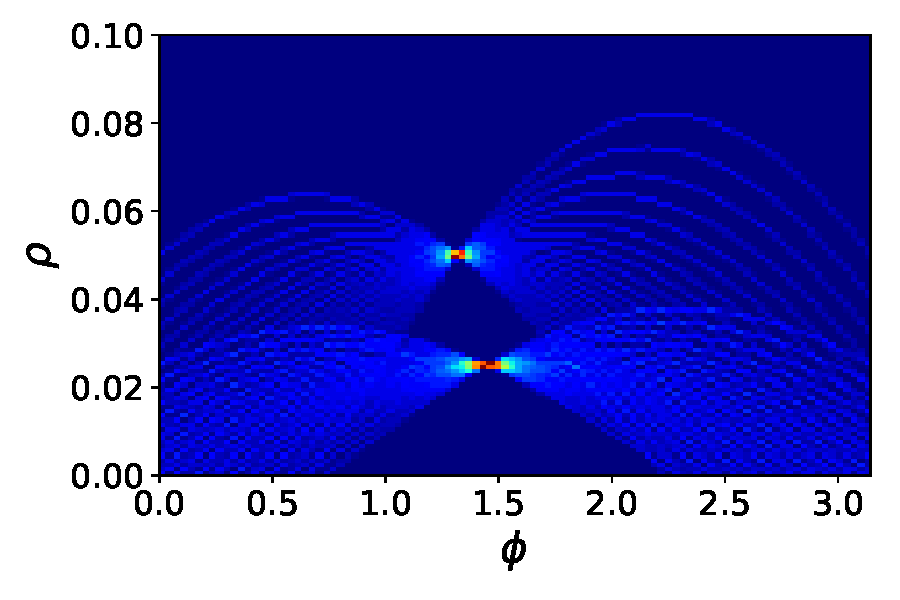
\includegraphics[width=\textwidth]{figures/circle_HT.pdf}
						\caption{}
				\end{subfigure}
	\label{HTcircle}
	\caption{Circles (a) as represented after a conformal mapping (b) and after the Hough transformation (c).}
\end{figure}

The Hough transformation is a periodic function and the points in the $\rho-\theta$ plane are bounded by $\theta \in \left[0, 2\pi\right]$ and $\rho \in \left[-\sqrt{u^2+v^2}, \sqrt{u^2+v^2}\right]$. It is important to note that the points $(\theta, \rho)$ and $(\theta+\pi, -\rho)$ describe the same line. In the studies presented in this document, to remove the ambiguity, $\rho$ is limited to positive values.


\subsubsection{Hough transform for helix}

\subsection{Hough transformation for particle tracks}
\subsection{Hough transformation for the incoherent pair background}
\subsection{Hough transformation and the simulation of jets}

For a center-of-mass energy of $\sqrt{s} = 91 \,\gev$, the simulation of the jets by the decay Z $\rightarrow$ d\={d}

\begin{figure}[ht]
	\centering
	\begin{subfigure}[b]{0.3\textwidth}
        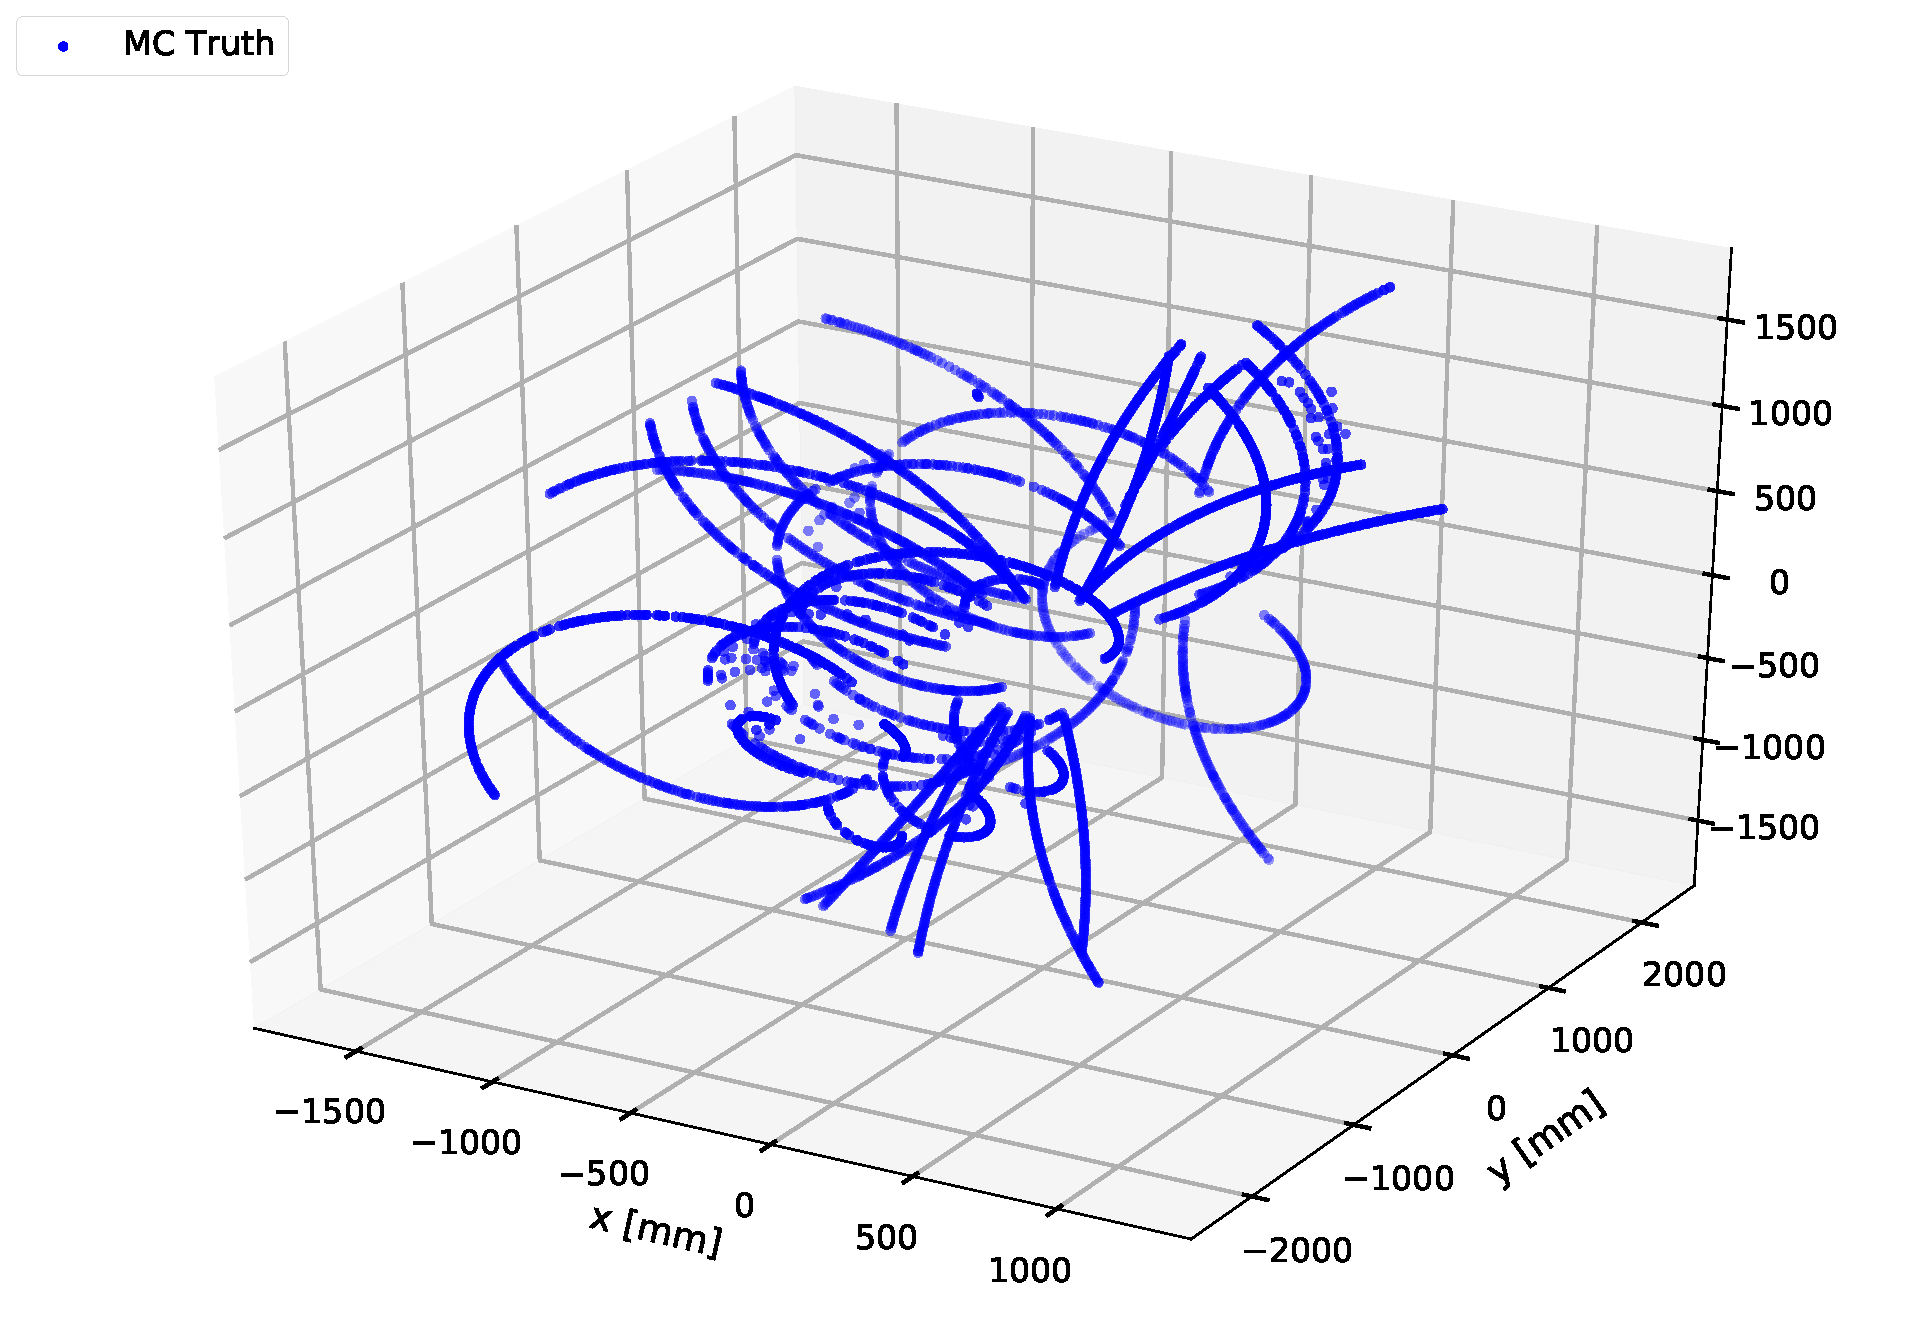
\includegraphics[width=\textwidth]{figures/Zdd_3D.pdf}
        \caption{}

    \end{subfigure}
		~ %
		\begin{subfigure}[b]{0.3\textwidth}
					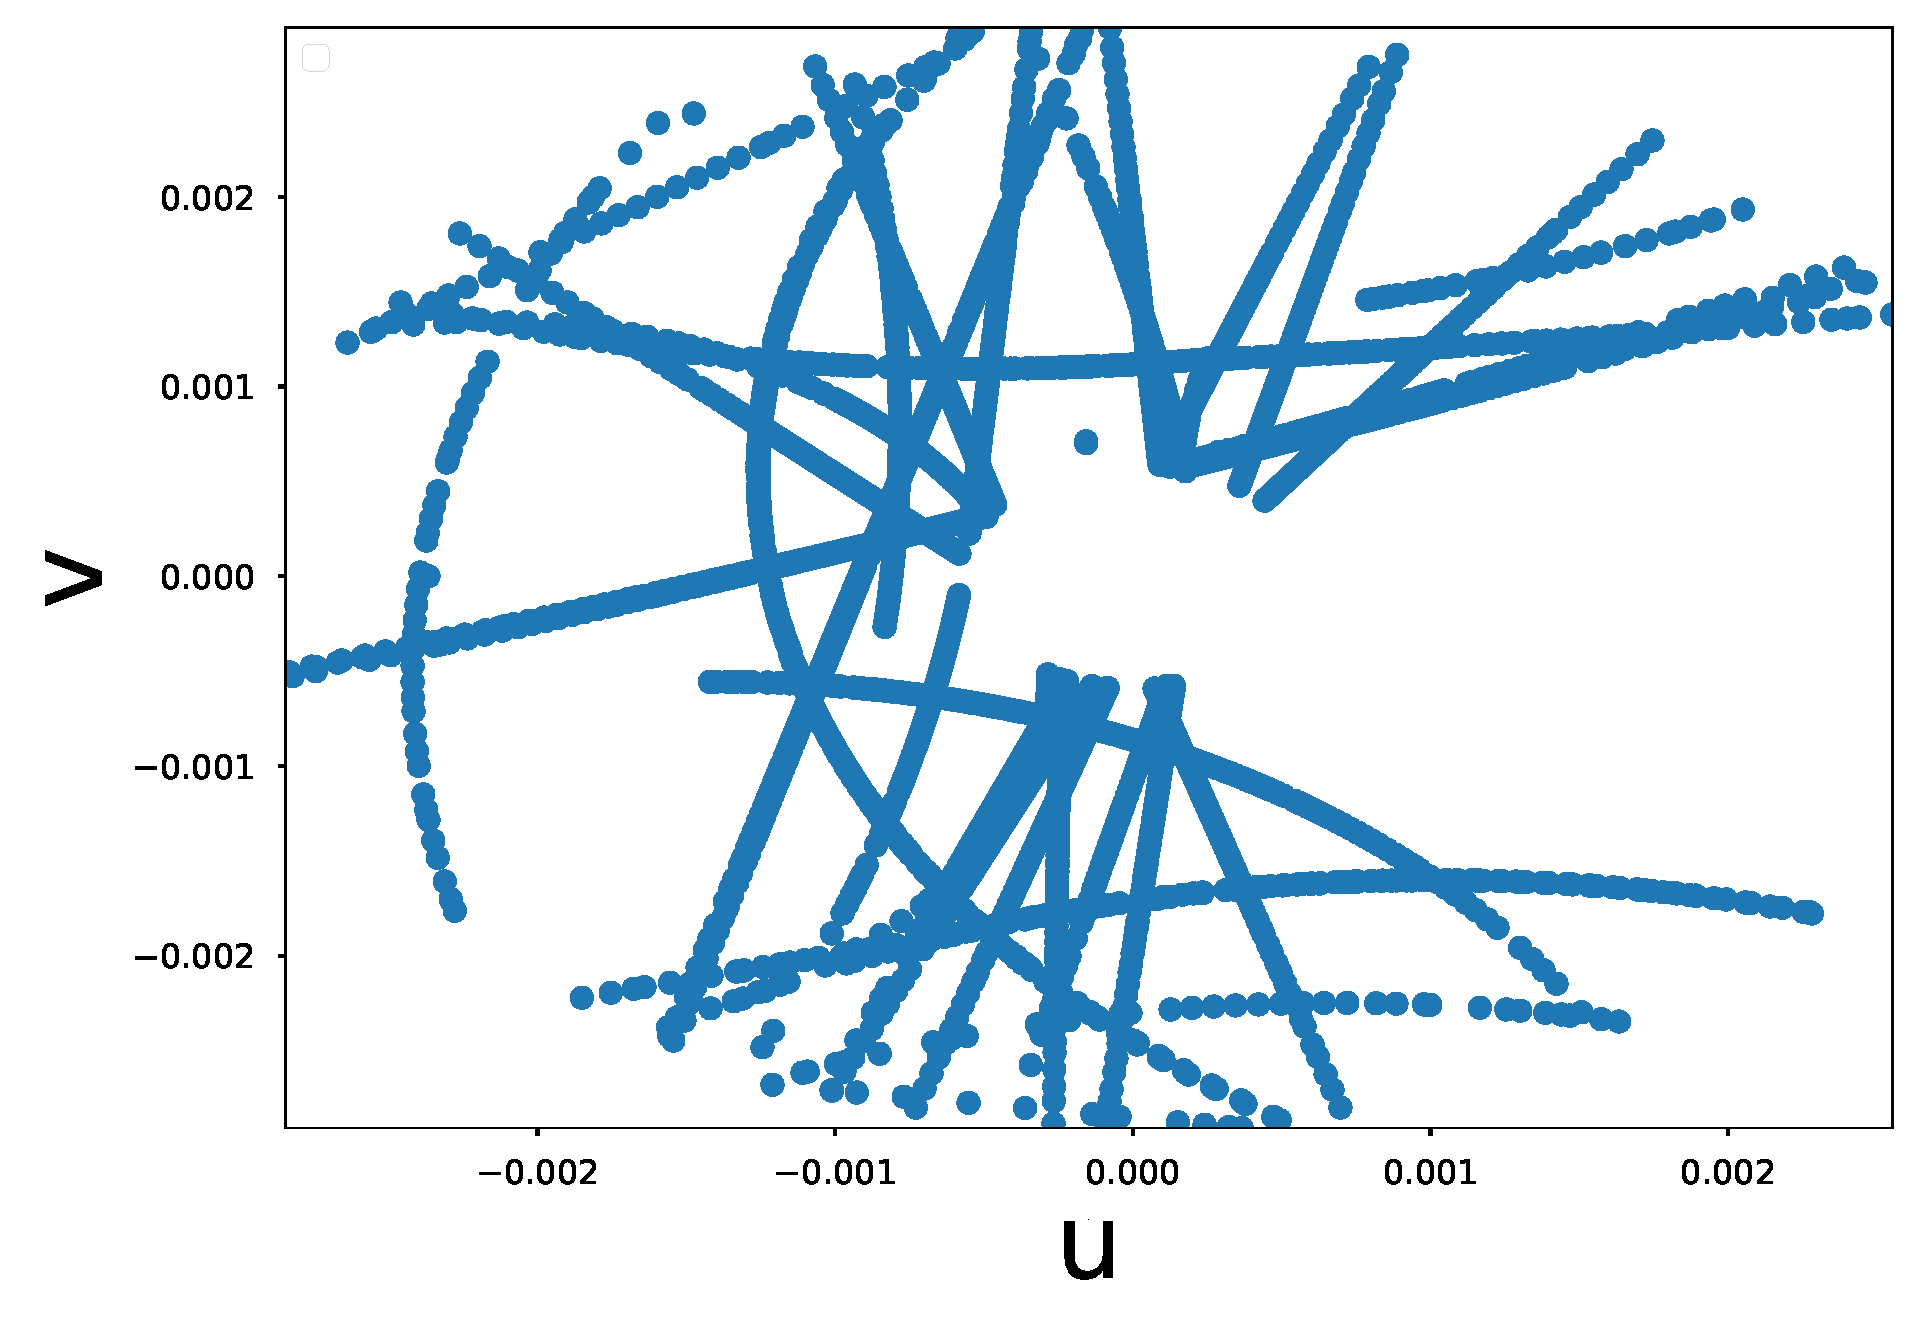
\includegraphics[width=\textwidth]{figures/CT_Zdd.pdf}
					\caption{}
			\end{subfigure}
			~ %
			\begin{subfigure}[b]{0.3\textwidth}
						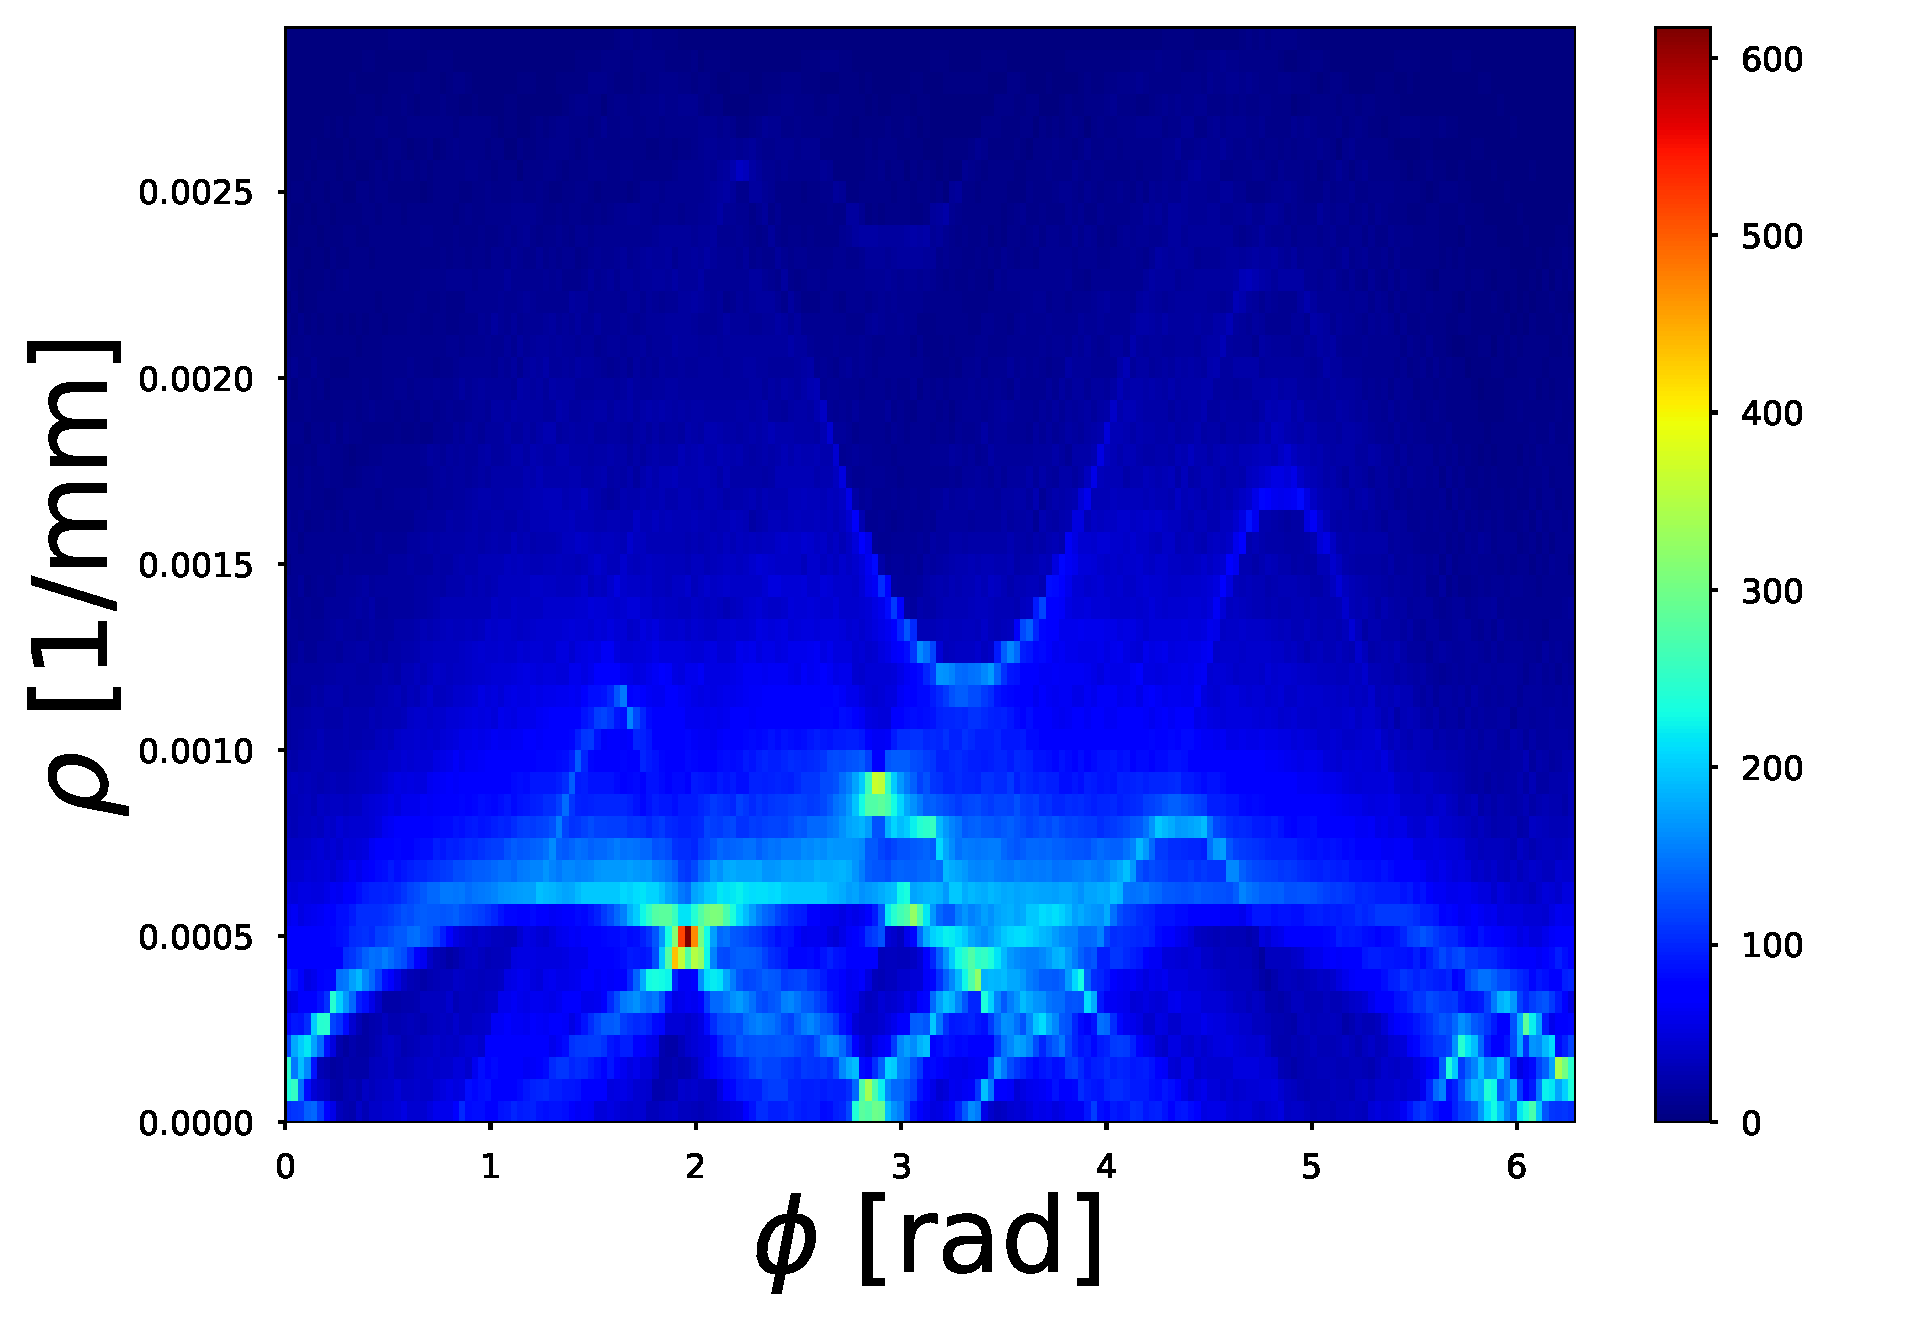
\includegraphics[width=\textwidth]{figures/HT_Zdd.pdf}
						\caption{}
				\end{subfigure}
	\label{HTZdd}
	\caption{Z $\rightarrow$ d\={d}}
\end{figure}
